\chapter{ Spread of Zika Virus on a Small World Network }

The deterministic models discussed in the chapters above assume that all individuals have an equally small probability of being infected. In this section we build a model for the propagation of Zika virus based on a small world network.

Traditional models of infectious disease dynamics have a long, successful history of describing and modelling infectious disease spread of many diseases. They are quiet simple and tractable \citep{fu2013propagation}.

There are certain specific and common situations when the structure of social connectivity is at least as important as the inactivity of the underlying infectious agents for the study of transmission of infection and control. This is one among the major reasons that has motivated the modelling of infectious diseases on social networks \cite{fu2013propagation}.



\section{ Vector Bone Disease Propagation on a Small World Network}
Assuming that there is a lattice with two layers. One for mosquitoes, another for human beings. We assume mosquitoes are stationary and that people have close and remote links. That is mosquitoes  do not cover long distances but just hover around a specific location. Where as people can travel to distant locations. Close links refer to individual's close acquaintances. 
 
A mosquito $M_1$ bites a Zika infected person $h_1$ with probability $\alpha_1$. Then transmits the virus to person $h_2$, with a probability of $\alpha_2$. Thus, person $h_1$ is connected to  person $h_2$ through $M_1$. It can then be said that $h_2$ can be infected by $h_1$ with probability $p_1$. Assuming that $\alpha_1 $ and $\alpha_2$ are independent  $p_1 =  \alpha_1 \alpha_2$. 
that $\alpha_1$ and $\alpha_2$.

 If person $h_3$ travels to the place where $h_1$ lives or gets close enough that he gets bitten by mosquito $M_1$ can be infected probability $\alpha_3$. Thus, $\alpha_3$ is the probability that person $h_3$ travels and get bitten by mosquito $M_1$. It can be said that $h_1$ infects $h_3$ with probability $p_2$, because $h_1$ is connected to $h_3$ through $M_1$. Assuming $\alpha_1$ and $\alpha_3$ are independent, $p_2 = \alpha_1 \alpha_3$.
\begin{figure}[h!]
\centering
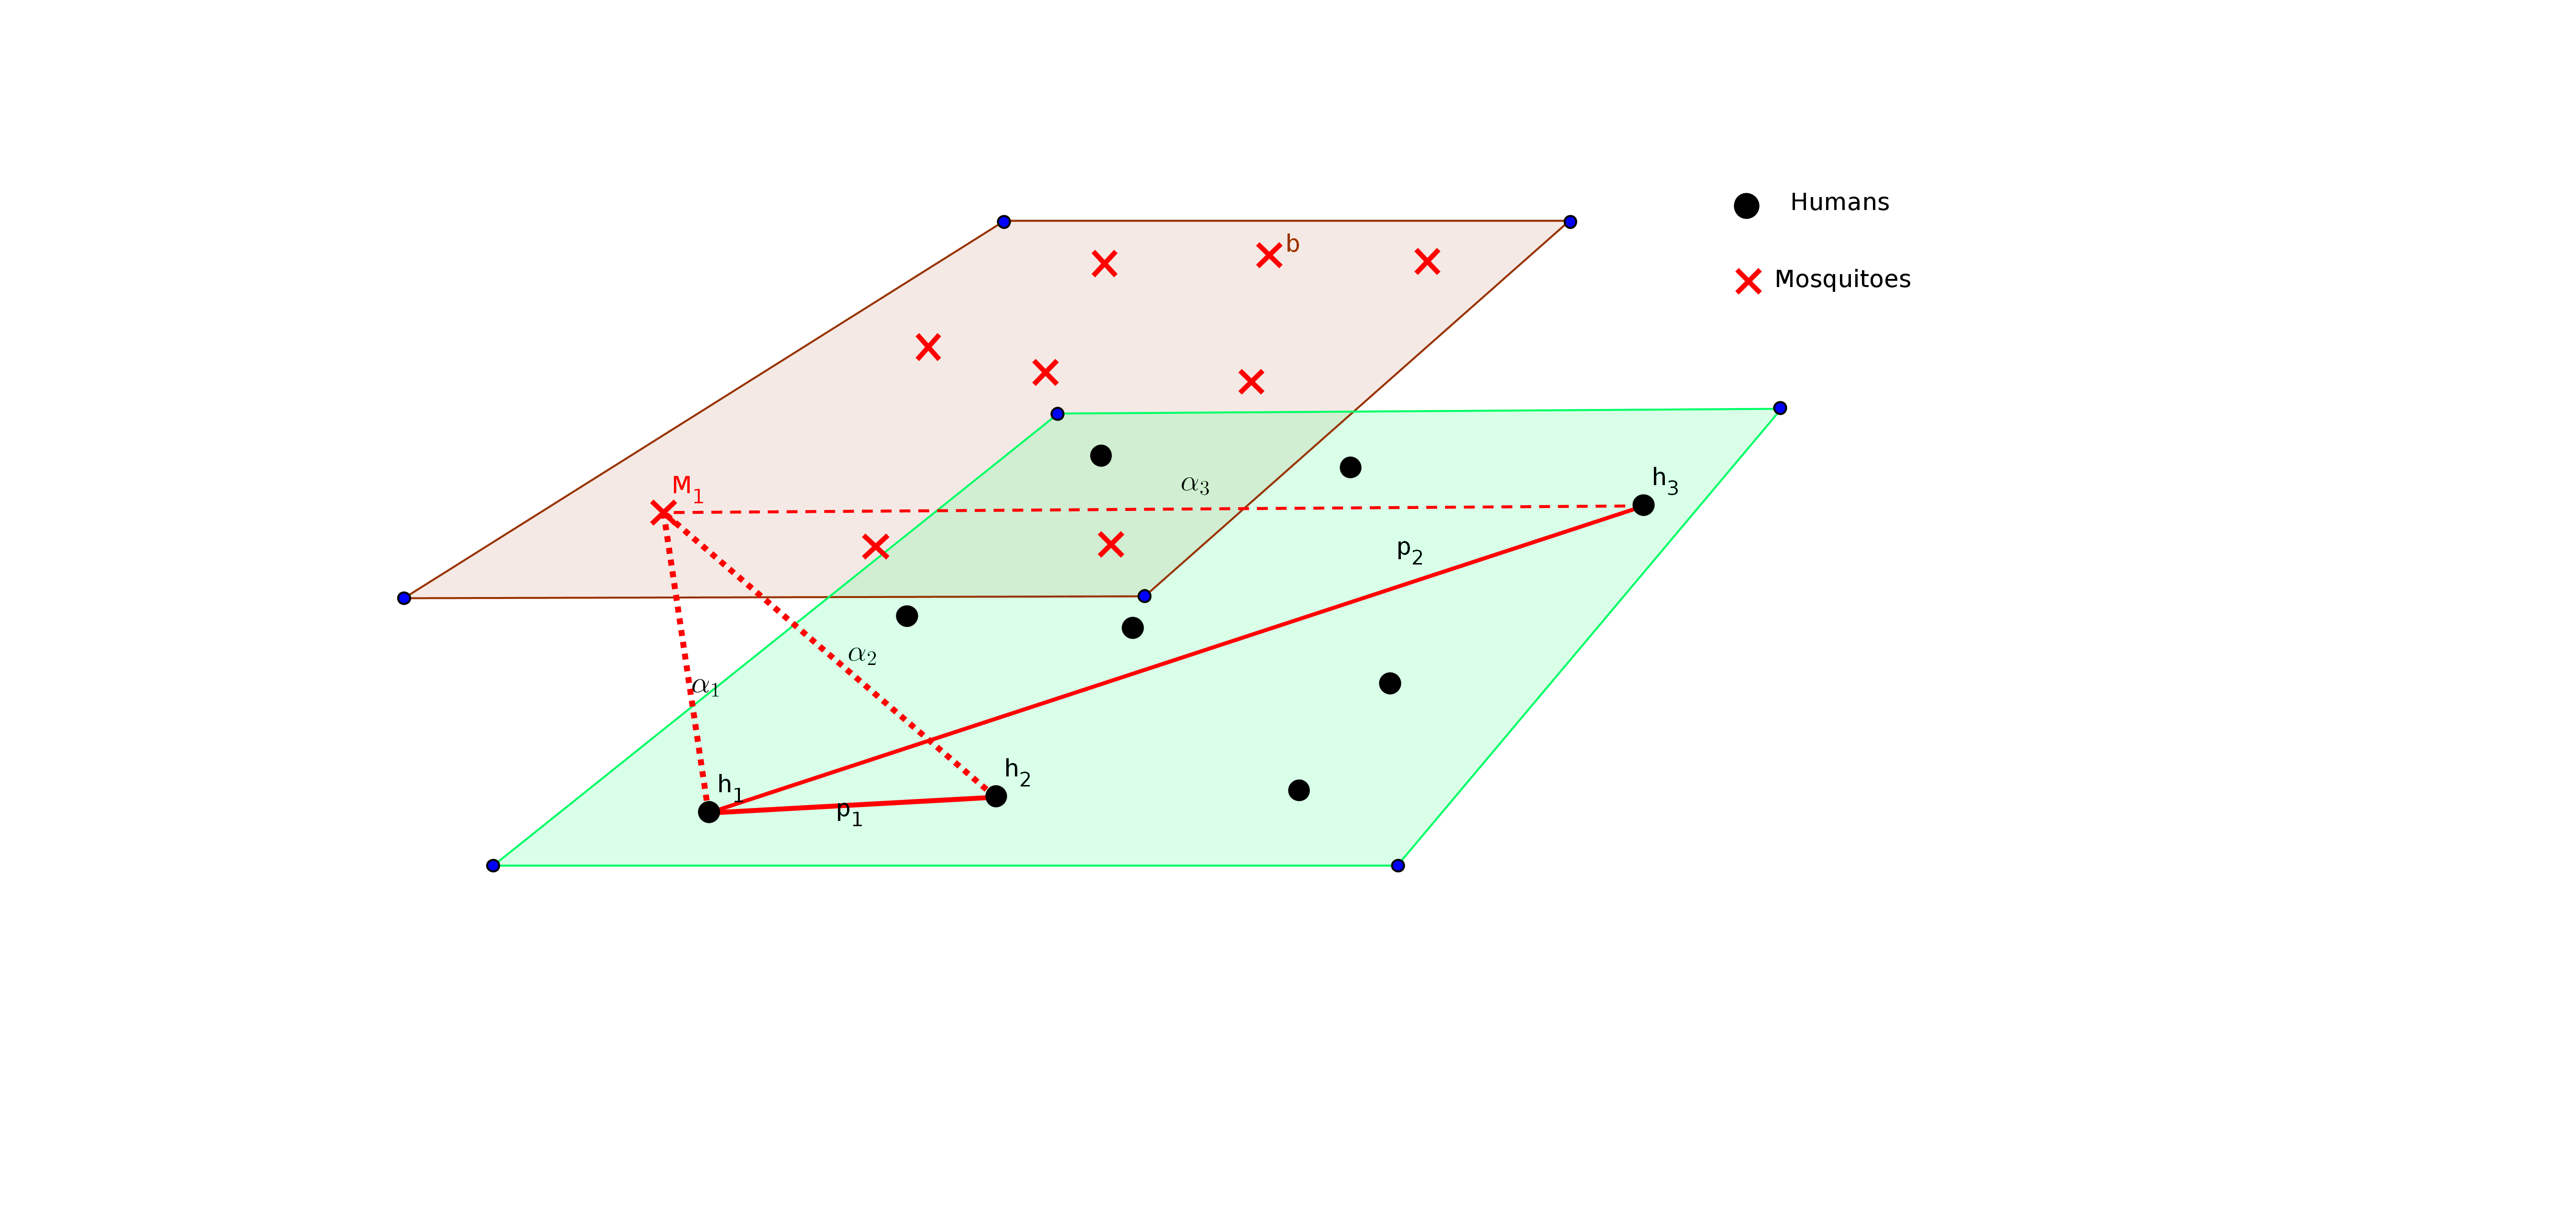
\includegraphics[scale=1]{images/human_mosquito.png}
\caption{Disease transmission through a vector} \label{fig5}
\end{figure}
The phenomenon of infecting a close like  or distant link can be expressed in 4 cases.


\begin{itemize}
\item[i.] $h_2$ may get infected by $h_1$ through $M_1$. In this case $h_1$ and $h_2$ are referred to as near neighbours.
\item[ii.] $h_4$ may travel to a place near enough to get the infection from $h_1$ through $M_1$. In this case $h_3$  referred to as a distant neighbour.
\item[iii.] $ h_1$ may travel to a place near enough to infect $h_4$  through another mosquito in that vicinity.In this case $h_3$ is  referred to as a distant neighbour.
\item[iv.] $h_1$  and $h_3$ may both travel to some place at the same time and $h_1$ transmits the infection to $h_3$ and this case is neglected. Thus for the this case $h_1$ and $h_3$ would no be referred to as near or distant neighbours.
\end{itemize}

In all the case we assume $\alpha_3$ is the same. Hence the probability of affecting a remote any distant neighbour neighbour is the same. We assume a single mosquito transmits at most   one infection. Thus $M_1$ is a scourge of mosquitoes.

The existence of near and distant neighbours in the disease infection dynamics of Zika virus on a lattice with two layers in \ref{fig5} makes it possible to represent the dynamics of disease spread on a small world network in figure \ref{fig 5.2}.Thus, in modelling the spread of Zika virus on a small world network, the dynamics of transmission through mosquitoes are represented by the edges of the graph. An edge is drawn between two vertices, whenever there is a likelihood of transmission from one to another via mosquito bite as can be seen in figure \ref{fig 5.2}.
\begin{figure}[h!]
\begin{minipage}[c]{1\textwidth}
 \centering
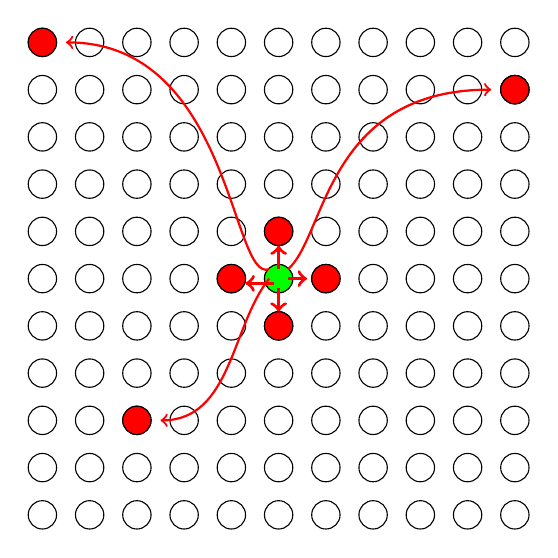
\begin{tikzpicture}[scale=0.6]
  \foreach \x in {0,...,10}
        \foreach \y in {0,...,10}
        {
        \draw (\x,\y) circle (0.3cm);
        }

\filldraw[fill=green!, draw=black](5,5) circle (0.3cm);
\filldraw[fill=red!, draw=black](2,2) circle (0.3cm);
\filldraw[fill=red!, draw=black](10,9) circle (0.3cm);
\filldraw[fill=red!, draw=black](10,9) circle (0.3cm);
\filldraw[fill=red!, draw=black](4,5) circle (0.3cm);
\filldraw[fill=red!, draw=black](5,4) circle (0.3cm);
\filldraw[fill=red!, draw=black](6,5) circle (0.3cm);
\filldraw[fill=red!, draw=black](5,6) circle (0.3cm);
\filldraw[fill=red!, draw=black](0,10) circle (0.3cm);

\draw[draw=red!,
preaction={->,thick,draw =red!}
] (5.2,5.2) ..controls(6,5.9) and (6,9) ..(9.5,9);
\draw[ draw =red!,thick, ->] (4.8,5.2) .. controls (4,4.9) and (4,10) ..(0.5,10);
\draw[ draw =red!,thick, ->] (4.8,5) .. controls (4,4) and (4,2) ..(2.5,2);
\draw[ draw =red!,very thick, ->] (5.2,5) -- (5.6,5);
\draw[ draw =red!,very thick, ->] (5,5.2) --(5,5.7);
\draw[ draw =red!,very thick, ->] (4.9,4.9) -- (4.3,4.9);
\draw[ draw =red!,very thick, ->] (5,4.8) --(5,4.3);
\end{tikzpicture}
%\caption{Smallworld network structure} \label{fig 5.1}
\end{minipage}
\caption{Smallworld network structure} \label{fig 5.1}
\end{figure}
\section{Small world methodology}

We  can now suppose that the population is arranged in a regular
2-dimensional square grid.  Where each vertex can infect its 4 nearest neighbours and a number of distant neighbours. Near neighbours in this case refers to individuals that one spends most of their time with, could be colleagues at work or school, people in the same house and distant neighbours refers to random individuals that one is likely to transmit the infection to. 
 
 \begin{figure}[h]
 \centering
 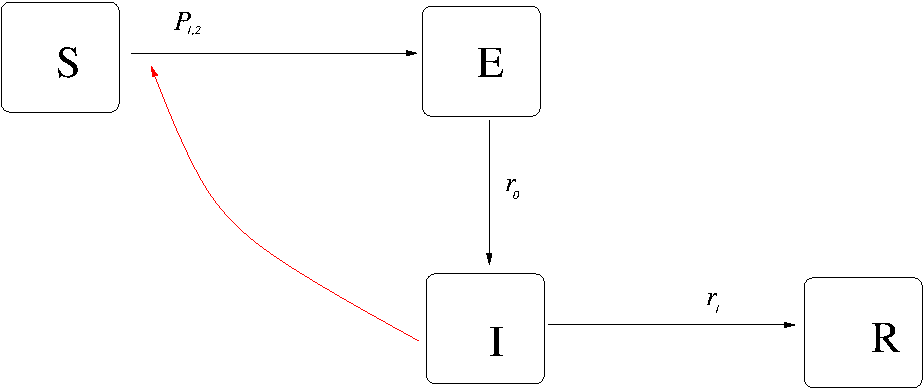
\includegraphics[scale=0.3]{images/swseir.png}
 \caption{State transition diagram} \label{fig 5.2}
\end{figure}
 
 
Figure \ref{fig 5.1} shows the arrangement of nodes in a small world network and figure \ref{fig 5.2} show the transmission state diagram: S to E based on the small world network structure and the infection probabilities $p_ {1,2} $: E to I with probability $r_0$ and I to R with probability $r_1$. in figure \ref{fig 5.1}, the infected green node may infect its four red near neighbours with probability $p_1$ and its three remote neighbours with probability $p_2$. By infection we mean transition from Susceptible to exposed state. 

Infected individuals can cause susceptible individuals, whom they are liked, to becomes exposed with with probability $p_1$ or $p_2$. Infected individuals can  infect their close neighbours with  probability $p_1$ and infect their distant neighbours with probability $p_2$. $p_1 $ and $p_2$ are probabilities of infection of per day. Infection in this case refers to the transition from susceptible to infected. Exposed individuals become infected with probability $r_0$ and infected individuals become recover with probability $r_1$.

The number of near neighbours $n_1 = 4$ or less, taking into account the boundary cases.
The number of distant neighbours $n_2$  for each node is independent and  identically distributed. That is for node each node $u$ there are $n_2^ {(u)} $ distant neighbours. $n_2^ {(u)} $ is chosen to follow a discrete exponentially decaying distribution 
\begin{equation} 
 \Pr[n_2^{(u)} = k] = c \cdot e^{-\mu x  } \label{5.2.1}
 \end{equation}
to remote nodes and $c = \dfrac{1}{1- e^{\frac{-1}{\mu}}}$ \citep{fu2013propagation}. The degree distribution in most social networks is exponentially distributed because of the celebrity effect \citep{estrada2015first}. In social networks, there are few people who have a high number of connections and many others with a few number of connections. In modelling infectious diseases these individuals are referred to as supper spreaders.

The transition probability $r_0$, the number of days an individual is in the exposed state is as a result a series of Bernoulli trials with mean $\frac{1}{r_0}$, follows a geometric distribution $f_X (x) = (1-p) ^ {x-1} p$. Similarly the infectious period follows a geometric distribution with mean $\dfrac{1}{r_o}$ \citep{fu2013propagation}.

\section{Model}
The model has seven parameters, they are $N, p_1, p_2, n_2, r_0$ and $r_1$. We let $N$ be the population size of a city or country and is arranged in a regular grid of side length $l $ such that $l^2 = N$. The rest of the parameters have been described above.

A thorough review of literature in \cite{lessler2016times} indicates that the incubation or latent period for Zika virus infection is $11.2$ days after infection with a $95 \%$ confidence interval of $7.6 -18$. Further the center for disease control and prevention (CDC) indicate that the incubation period for the Zika virus ranges from 3 days to 14 days from infection \citep{krow2017estimated}. Therefore we estimate $r_o$ with $\frac{1}{11.2}$
  \Jnote{These are the values before you exhibit symptoms. Are they the same
    for becoming infective?}
  \Jnote{Consider adding some days to allow time for a mosquito to transmit  the virus.}

  $95\%$ of the cases will still have detectable virus infectiousness 18.9 days after infection with a confidence interval of 13.6 -79.4 \citep{lessler2016times}.The infectiousness in Zika infection ends 1.5 - 2 days before the virus becomes undetectable \citep{funk2016comparative}. Thus the chosen value of the infectious period is $18.9 - 1.5 = 17.4$ days. Therefore $r_1$ is estimated to be $\dfrac{1}{17.4}$.

Hence we have $\mu$, $p_1$ and $p_2$ free parameters. Without active control, the average number of secondary infections resulting from a primary  Zika  virus infectious is between 3 and 6, therefore we choose 4.5 as the $R_0$. Since the number of remote neighbours is random and fixed for each, we estimate $E (n^ {(u)} _2) = \mu$.

In this state each infectious individual will infect on average $n_1p_1 + E[n^(u)]p_2 $ new individuals everyday. The average number  of individuals infected each day can be estimated by the number of secondary infections each day of an individuals infectious period. Thus ;
\begin{align}
n_1 p_1 + \mu p_2 \approx \dfrac{R_0}{r_1} 
\\ n_1 p_1 + \mu p_2 \approx 0.2586 \label{eqn 5.32}
\end{align}
thus, 
$p_1 \approx   0.0645- 0.25 \mu p_2$ , in terms of small world parameters $\mu$ and $p_2$.

Now $n_1$ and $n_2$ represent the number of interactions an individual has each day. Hence the  $n_1 + n_2$ is the lower bound is a lower bound of the number of active acquaintances because it is a number of link that are sufficiently intimate to support transmission of the virus. In reality some links would be closer than other and more likely to lead to transmission. We assume that all $n_1$ links are infected with probability $p_1$ and $n_2$ with probability $p_2$ each day. The probability $p_1$ and $p_2$ are not the same.

Note that the choice of $n_1$ and $n_2$ is not critical; what is more important is the infection probability $n_1p_1 + n_2p_1$ .

We can summarize the parameters of the models as;
\begin{align}
n_1 &= 4 \\
\mu &= 8 \\
r_0 &= \dfrac{1}{11.2} \approx 0.089 \\
r_1 &= \dfrac{1}{17.4} \approx 0.057 \\
p_1 &= 0.0645 - 2 p_2 \label{eqn 5.1.7}
\end{align}
Now we have one free parameter $p_2$. We can now estimate the number of new infections by;
\begin{align}
E(- \bigtriangleup S) = (n_1 k p_1 + \mu p_2 - r_1) I \label{5.18}
\end{align}
Where k is the average number of near neighbours' links that support possible infection and near neighbours are arranged in clusters, therefore $0.5 k 1$.  In our computation, we will take $k = 0.5$. From equation \ref{5.18} we can estimate the number of new infections as;
\begin{align}
E(- \bigtriangleup S) = (2 p_1 + 8 p_2 - 0.057) I  \label{5.1.9}
\end{align}
 
From equation \ref{eqn 5.32}, it can be shown that $p_1$ and $p_2$ have natural bounds. That is taking $p_2 = 0$, implies that $p_1 \leq 0.1293$ for $k =0. 5$. For $p_1 = 0$, we get $p_2 \leq 0.3232$.
\section{Simulation}
To investigate how disease propagation varies depending on $p_1, p_2, $ and $r_1$ we ran a couple of simulations on a small work network. 

We initiate the model with one infected individual and an $r_1$ which is relatively small .As the  infection progresses  we increase $r_1$ to reflect changes in health care as a response to the Zika out break. We assume the other parameter are constant.

\section{Results}

\begin{figure}
\centering
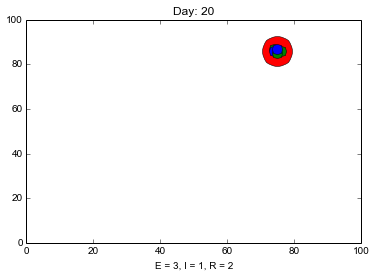
\includegraphics[scale=0.25]{images/1t20.png} \quad
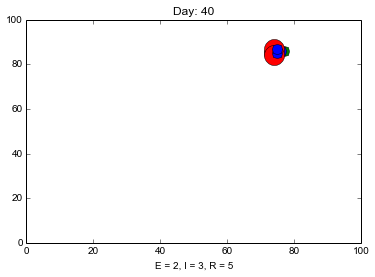
\includegraphics[scale=0.25]{images/1t40.png} \quad
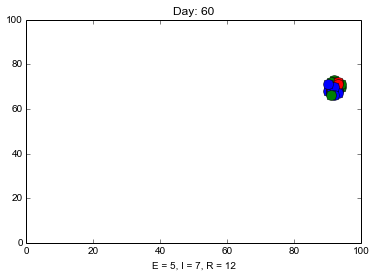
\includegraphics[scale=0.25]{images/1t60.png} \quad
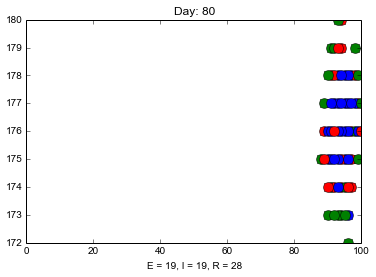
\includegraphics[scale=0.25]{images/1t80.png} 

\medskip
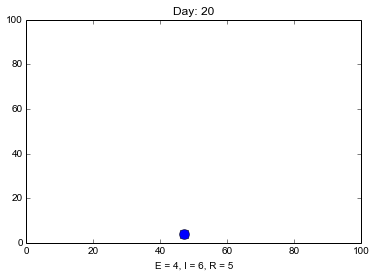
\includegraphics[scale=0.25]{images/2t20.png} \quad
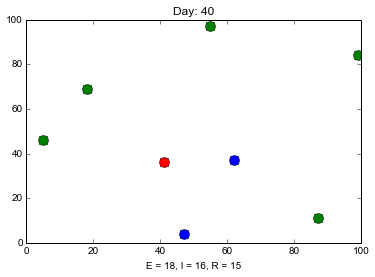
\includegraphics[scale=0.25]{images/2t40.png} \quad
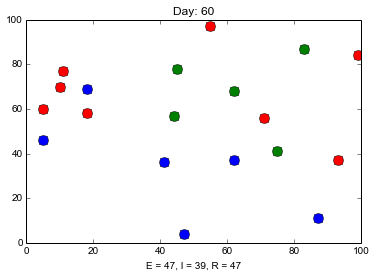
\includegraphics[scale=0.25]{images/2t60.png} \quad
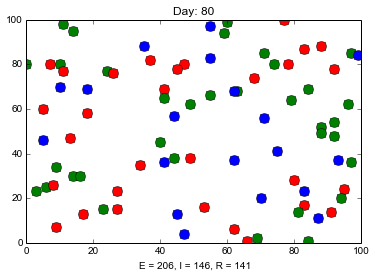
\includegraphics[scale=0.25]{images/2t80.png} 

\medskip
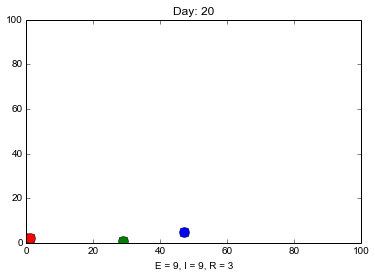
\includegraphics[scale=0.25]{images/3t20.png} \quad
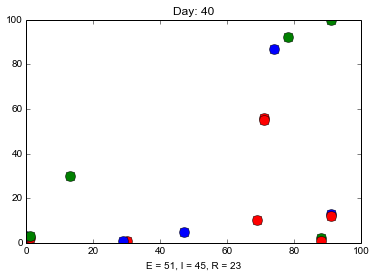
\includegraphics[scale=0.25]{images/3t40.png} \quad
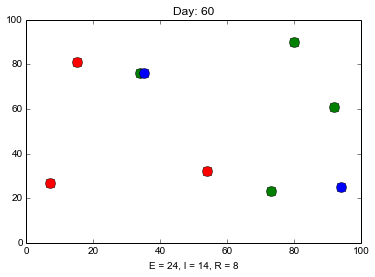
\includegraphics[scale=0.25]{images/3t60.png} \quad
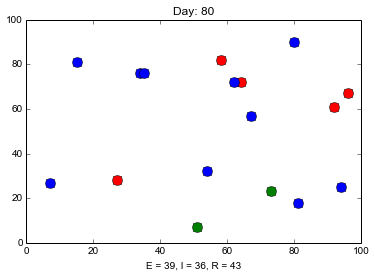
\includegraphics[scale=0.25]{images/3t80.png} 

\medskip
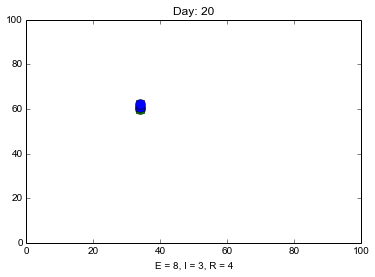
\includegraphics[scale=0.25]{images/4t20.png} \quad
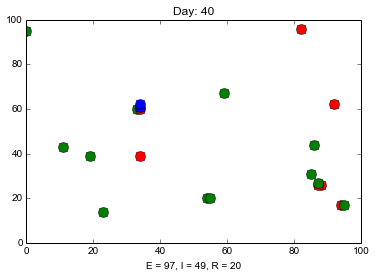
\includegraphics[scale=0.25]{images/4t40.png} \quad
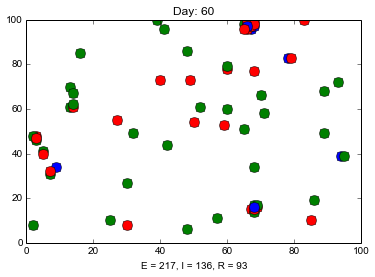
\includegraphics[scale=0.25]{images/4t60.png} \quad
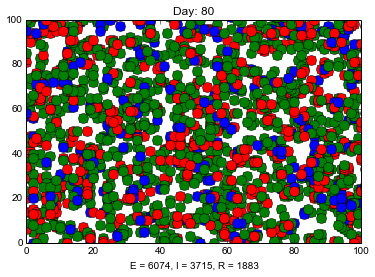
\includegraphics[scale=0.25]{images/4t80.png} 

\medskip
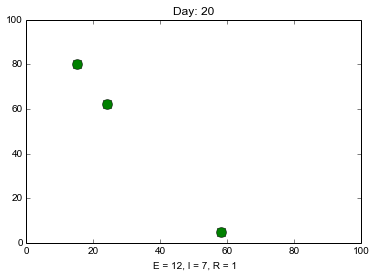
\includegraphics[scale=0.25]{images/5t20.png} \quad
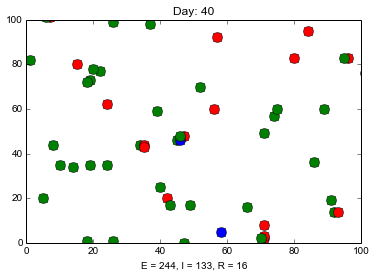
\includegraphics[scale=0.25]{images/5t40.png} \quad
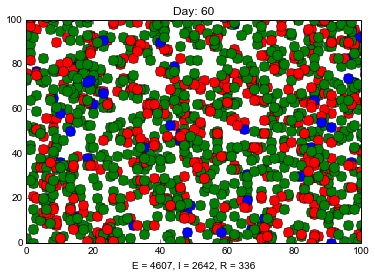
\includegraphics[scale=0.25]{images/5t60.png} \quad
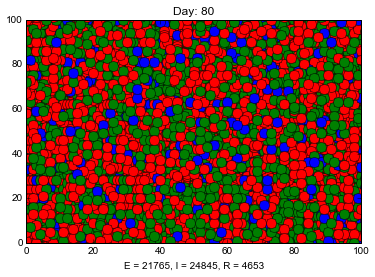
\includegraphics[scale=0.25]{images/5t80.png} 
\end{figure}
